\documentclass[letterpaper,10pt]{article}

\setlength{\evensidemargin}{-0.0in}
\setlength{\oddsidemargin}{-0.0in}
\setlength{\textwidth}{6.4in}

\usepackage[utf8]{inputenc}
\usepackage{amsmath}
\usepackage{amssymb}
\usepackage{enumerate}
\usepackage{mathpazo}
\usepackage{relsize}
\usepackage{mathtools}
\usepackage{mathrsfs}
\usepackage{verbatim}

\usepackage{hyperref}
\hypersetup{
    colorlinks=true,
    linkcolor=blue,
    filecolor=magenta,      
    urlcolor=blue,
}

\usepackage{tikz}
\usetikzlibrary{matrix,arrows}

\usepackage{fancyhdr}
\pagestyle{fancy}
\lhead{Seshadri's First Main Lemma}
\rhead{Tuomas Tajakka}
%\cfoot{}
\rfoot{}
\renewcommand{\headrulewidth}{0.4pt}

\usepackage{amsthm}

\newtheorem{thm}{Theorem}[section]
\newtheorem{lem}[thm]{Lemma}
\newtheorem{prop}[thm]{Proposition}
\newtheorem{cor}[thm]{Corollary}
\newtheorem{expl}[thm]{Example}
\newtheorem{defn}[thm]{Definition}

\theoremstyle{remark}
\newtheorem{rmk}[thm]{Remark}
\newtheorem{exer}[thm]{Exercise}

\title{Seshadri's First Main Lemma}
\author{Tuomas Tajakka}
\date{}

\usepackage{commands}


\begin{document}

\maketitle

\section{Introduction}
In this note we give a proof of a refined version of Lemma 3.1 (First Main Lemma) in \cite{seshadri}. Let $k$ be an algebraically closed field, $C$ a smooth, projective, connected curve of genus $g \ge 2$ over $k$, and let $F$ be a stable vector bundle on $C$. Our main result is the following theorem.

\begin{thm}
    Let $r$ be an integer greater than $\rk(F)$ and invertible in $k$, and let $\sL$ be a line bundle of degree $d$ on $C$. Assume that
    \[ d \rk(F) + r \deg(F) + r \rk(F) (1-g) = 0. \]
    There exists a vector bundle $E$ on $C$ such that $\rk(E) = r, \det(E) = \sL$, and 
    \[ H^0(C, E \otimes F) = H^1(C, E \otimes F) = 0. \]
\end{thm}
Note that the condition
\[ \deg(E) \rk(F) + \rk(E) \deg(F) + \rk(E) \rk(F) (1-g) = 0 \]
is by the Riemann-Roch theorem equivalent to
\[ \chi(X, E \otimes F) = H^0(X, E \otimes F) - H^1(X, E \otimes F) = 0. \]

\section{Proof}
We prove the contrapositive. In other words, we assume that \emph{there does not exist a vector bundle $E$ of rank $r$ and determinant $\sL$ such that} 
\[ H^0(X, E \otimes F) = H^1(X, E \otimes F) = 0, \]
and construct a destabilizing subsheaf of $F$.

Let $S$ be a finite type miniversal deformation space of simple vector bundles of rank $r$ and determinant $\sL$. It is smooth over $k$ and irreducible of dimension $(r^2 - 1)(g-1)$. Denote by $p: S \times X \to S$ and $q: S \times X \to X$ the projections. In the course of the argument, we will repeatedly replace $S$ be open subspaces.

Let $\sE$ be a coherent sheaf on $S \times X$ flat over $S$. For a closed point $t \in S$, denote by $\sE_t$ the the restriction of $\sE$ to the fiber $p^{-1}(t) \cong X$. There is a canonical linear map
\[ \ka: T_{S,t} \otimes H^0(X, \sE_t) \to H^1(X, \sE_t) \]
defined as follows. View a tangent vector $v \in T_{S,t}$ as a morphism $v: \Spec k[\eps] \to S$ that takes the unique point of $\Spec k[\eps]$ to $t$. Denote by $j: X \to X_\eps \coloneqq X \times \Spec k[\eps]$ the closed embedding given by $\eps \mapsto 0$, and by $v_X = v \times \id_X: X_\eps \to S\times X$ the product map.

\begin{center}
    \begin{tikzpicture}
    \matrix (m) [matrix of math nodes, row sep=4em, column sep=4em]
    { \sE_t & v_X^* \sE & \sE & \\ 
    X & X_\eps & S \times X & X \\
    \Spec k & \Spec k[\eps] & S & \\};
    \path[->] 
    (m-2-1) edge node[auto] {$ j $} (m-2-2)
    (m-2-1) edge node[auto] {$  $} (m-3-1)
    (m-2-2) edge node[auto] {$ v_X $} (m-2-3)
    (m-2-2) edge node[auto] {$ $} (m-3-2)
    (m-2-3) edge node[auto] {$ q $} (m-2-4)
    (m-2-3) edge node[auto] {$ p $} (m-3-3)
    (m-3-1) edge node[auto] {$ \eps \mapsto 0 $} (m-3-2)
    (m-3-2) edge node[auto] {$ v $} (m-3-3)
    ;
    {\color{red} Do it.}
    (m-1-1) edge node[auto] {$  $} (m-2-1)
    (m-1-2) edge node[auto] {$  $} (m-2-2)
    (m-1-3) edge node[auto] {$  $} (m-2-3)
    ;        
    \end{tikzpicture}
\end{center}

Now $v_X^*\sE$ is flat over $\Spec k[\eps]$ and so fits in an exact sequence
\[ 0 \to j_* \sE_t \to v_X^*\sE \to j_* \sE_t \to 0 \]
of sheaves on $X_\eps$. The connecting homomorphism in the exact sequence in sheaf cohomology
\[ H^0(X, \sE_t) = H^0(X_\eps, j_*\sE_t) \to H^1(X_\eps, j_*\sE_t) = H^1(X, \sE_t) \]
gives the map $\ka(v, -)$. If $p_*\sE$ is locally free on $S$ and its formation commutes with arbitrary base change, then the map
\[ H^0(X_\eps, v_X^*\sE) \to H^0(X, \sE_t) \]
is identified with the \emph{surjective} evaluation-at-$t$ map $(p_*\sE) \otimes k[\eps] \to (p_* \sE) \otimes k$, and so the connecting homomorphism above is the zero map, and hence so is $\ka$. 

From now on, we denote by $\sE$ the \emph{universal vector bundle} on $S \times X$. The canonical evaluation map $\sE^\vee \otimes \sE \to \Oh_{S \times X}$, also called the trace map, has a section $\Oh_{S \times X} \to \sHom(\sE, \sE) \cong \sE^\vee \otimes \sE$ given by $1 \mapsto 1/r \cdot \id_{\sE}$. \emph{This is where we need $r$ to be invertible in $k$}. Thus, we have a split exact sequence
\[ 0 \to \sA \to \sE^\vee \otimes \sE \xrightarrow{\mathrm{tr}} \Oh_{S \times X} \to 0, \]
where $\sA$, the "sheaf of traceless endomorphisms", is locally free. For a closed point $t \in S$, we obtain a split exact sequence
\[ 0 \to \sA_t \to \sE_t^\vee \otimes \sE_t \to \Oh_X \to 0, \]
and in cohomology
\begin{equation} \label{H1exact}
    0 \to H^1(X, \sA_t) \to H^1(X, \sE_t^\vee \otimes \sE_t) \to H^1(X, \Oh_X) \to 0.
\end{equation}
The vector space $H^1(X, \sA_t)$ \emph{is naturally isomorphic to the tangent space} $T_{S,t}$. 

Consider the sheaf $\sE \otimes q^*F$ on $S \times X$. Recall that the assumption
\[ d \rk(F) + r \deg(F) + r \rk(F) (1-g) = 0 \]
implies that 
\[ \chi(X, \sE_t \otimes F) = H^0(X, \sE_t \otimes F) - H^1(X, \sE_t \otimes F) = 0 \] 
for all $t \in S$. The function $S \to \N, t \mapsto \dim H^0(X, \sE_t \otimes F) = \dim H^1(X, \sE_t \otimes F)$ is upper semicontinuous and so takes a constant minimal value over an open subspace of $S$. \emph{We replace $S$ by this open subspace.} After this replacement, Grauert's theorem implies that the sheaves $p_*(\sE \otimes q^*F)$ and $R^1 p_*(\sE \otimes q^*F)$ are locally free and their formation commutes with base change. In particular, their fibers at $t \in S$ are naturally identified with 
\[ H^0(X, \sE_t \otimes F) \qquad \mathrm{and} \qquad H^1(X, \sE_t \otimes F) \] respectively.

For the sheaf $\sE \otimes q^*F$, the map $\ka$ constructed above coincides with the composition
\begin{equation}\label{kappa}
H^1(X, \sA_t) \otimes H^0(X, \sE_t \otimes F) \to H^1(X, \sE_t^\vee \otimes \sE_t) \otimes H^0(X, \sE_t \otimes F) \to H^1(X, \sE_t \otimes F)
\end{equation}
under the identification of $T_{S,t}$ with $H^1(X, \sA_t)$, where the first map is induced by the inclusion 
\[ H^1(X, \sA_t) \hookrightarrow H^1(X, \sE_t^\vee \otimes \sE_t) \] 
and the second map can be expressed using the derived category as
\begin{center}
    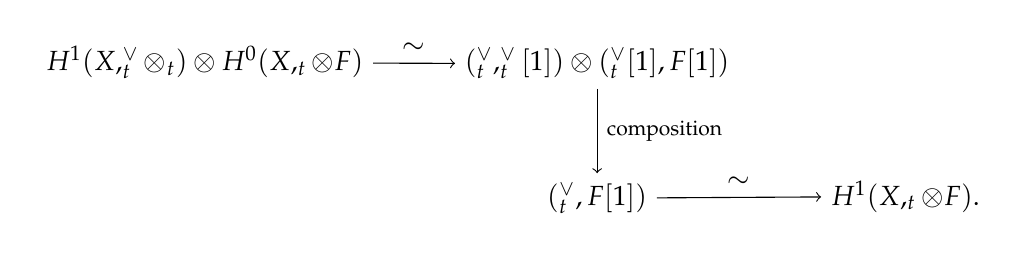
\begin{tikzpicture}
    \matrix (m) [matrix of math nodes, row sep=3em, column sep=3em]
    { H^1(X, \sE_t^\vee \otimes \sE_t) \otimes H^0(X, \sE_t \otimes F) & \Hom(\sE_t^\vee, \sE_t^\vee[1]) \otimes \Hom(\sE_t^\vee[1], F[1]) & \\
    & \Hom(\sE_t^\vee, F[1]) & H^1(X, \sE_t \otimes F). \\};
    \path[->] 
    (m-1-1) edge node[auto] {$ \sim $} (m-1-2)
    (m-1-2) edge node[auto] {$ _\mathrm{composition} $} (m-2-2)
    (m-2-2) edge node[auto] {$ \sim $} (m-2-3)
    ;        
    \end{tikzpicture}
\end{center}
As we saw above, since $p_*(\sE \otimes q^*F)$ is locally free and its formation commutes with base change, the map (\ref{kappa}) is the zero map. Using Serre duality and tensor-hom adjunction, we see that (\ref{kappa}) is adjoint to the map
\[ \Hom(\sE_t^\vee, F) \otimes \Hom(F, \sE_t^\vee \otimes \om_X) \to H^0(X, \sA_t^\vee \otimes \om_X) \]
fitting in the diagram
\begin{center}
    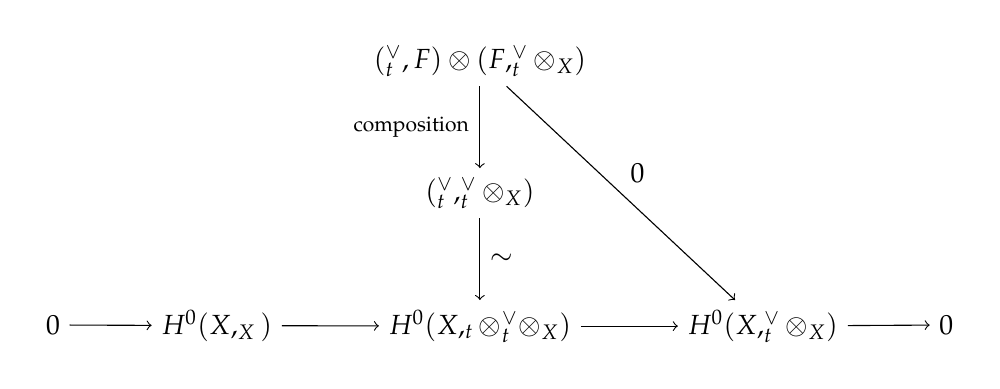
\begin{tikzpicture}
    \matrix (m) [matrix of math nodes, row sep=3em, column sep=3em]
    { & & \Hom(\sE_t^\vee, F) \otimes \Hom(F, \sE_t^\vee \otimes \om_X) & & \\
      & & \Hom(\sE_t^\vee, \sE_t^\vee \otimes \om_X) & & \\
    0 & H^0(X, \om_X) & H^0(X, \sE_t \otimes \sE_t^\vee \otimes \om_X) & H^0(X, \sA_t^\vee \otimes \om_X) & 0 \\};
    \path[->] 
    (m-1-3) edge node[auto,swap] {$ _\mathrm{composition} $} (m-2-3)
    (m-1-3) edge node[auto] {$ 0 $} (m-3-4)
    (m-2-3) edge node[auto] {$ \sim $} (m-3-3)
    (m-3-1) edge node[auto] {$  $} (m-3-2)
    (m-3-2) edge node[auto] {$  $} (m-3-3)
    (m-3-3) edge node[auto] {$  $} (m-3-4)
    (m-3-4) edge node[auto] {$  $} (m-3-5)
    ;        
    \end{tikzpicture}
\end{center}
where the bottom sequence is Serre dual to (\ref{H1exact}).

This diagram is saying that every composition $\sE_t^\vee \to F \to \sE_t^\vee \otimes \om_X$ arises uniquely from a section $\si: \Oh_X \to \om_X$ as 
\[ \sE_t^\vee \xrightarrow{\id \otimes \si} \sE_t^\vee \otimes \om_X. \] 
\emph{Now we use the assumption that $\rk(\sE) > \rk(F)$.} Notice that any nonzero section $\Oh_X \to \om_X$ is injective, and since $\sE_t$ is locally free, also $\sE_t^\vee \to \sE_t^\vee \otimes \om_X$ is injective. But $\sE_t^\vee \to F$ cannot be injective, hence neither can $\sE_t^\vee \to F \to \sE_t^\vee \otimes \om_X$. We conclude that \emph{the map}
\[ \Hom(\sE_t^\vee, F) \otimes \Hom(F, \sE_t^\vee \otimes \om_X) \to \Hom(\sE_t^\vee, \sE_t^\vee \otimes \om_X) \]
\emph{is the zero map.}

Let $\sG$ and $\sQ$ denote respectively the image and cokernel of the canonical evaluation map
\[ p^*p_*\sHom(\sE^\vee, q^*F) \otimes \sE^\vee \longrightarrow q^*F \]
adjoint to $p_*(\sE \otimes q^*F) \xrightarrow{\id} p_*(\sE \otimes q^*F)$. There is a nonempty open subspace of $S$ over which 
\begin{enumerate}[(i)]
    \item $\sG$ and $\sQ$ are flat, and
    \item the dimension of $H^0(X, \sE_t \otimes \sG_t)$ remains constant.
\end{enumerate} 
\emph{We replace $S$ by this open subspace.} As a result, $\sG$ and $\sQ$ are flat over $S$, and $p_*(\sE \otimes \sG)$ is locally free on $S$ and its formation commutes with base change. Moreover, the restriction $\sG_t$ of $\sG$ to the fiber over $t \in S$ identifies with the image of the evaluation map $\Hom(\sE_t^\vee, F) \otimes \sE_t^\vee \to F$. 

By assumption we have $H^0(X, \sE_t \otimes F), H^1(X, \sE_t \otimes F) \neq 0$. Now by construction
\[ \Hom(\sE_t^\vee, \sG_t) \cong \Hom(\sE_t^\vee, F) \cong H^0(X, \sE_t \otimes F) \neq 0, \]
so in particular $\sG_t \neq 0$. Moreover, denoting $V = \Hom(\sE_t^\vee, F)$ and applying $\Hom(-, \sE^\vee \otimes \om_X)$ to the diagram
\begin{center}
    \begin{tikzpicture}
    \matrix (m) [matrix of math nodes, row sep=3em, column sep=3em]
    { & V \otimes \sE_t^\vee & & & \\
    0 & \sG_t & F & \sQ_t & 0 \\};
    \path[->>] 
    (m-1-2) edge node[auto,swap] {$  $} (m-2-2)
    ;
    \path[->]
    (m-2-1) edge node[auto,swap] {$  $} (m-2-2)
    (m-2-2) edge node[auto,swap] {$  $} (m-2-3)
    (m-2-3) edge node[auto,swap] {$  $} (m-2-4)
    (m-2-4) edge node[auto,swap] {$  $} (m-2-5)
    ;        
    \end{tikzpicture}
\end{center}
where the horizontal sequence is exact and the vertical map is surjective, we obtain a diagram
\begin{center}
    \begin{tikzpicture}
    \matrix (m) [matrix of math nodes, row sep=3em, column sep=3em]
    { 0 & \Hom(\sQ_t, \sE_t^\vee \otimes \om_X) & \Hom(F, \sE_t^\vee \otimes \om_X) & \Hom(\sG_t, \sE_t^\vee \otimes \om_X) \\
    & & & \Hom(V \otimes \sE_t^\vee, \sE_t^\vee \otimes \om_X)\\
    };
    \path[->] 
    (m-1-1) edge node[auto,swap] {$  $} (m-1-2)
    (m-1-2) edge node[auto,swap] {$  $} (m-1-3)
    (m-1-3) edge node[auto,swap] {$  $} (m-1-4)
    ;
    \path[right hook ->]
    (m-1-4) edge node[auto,swap] {$  $} (m-2-4)
    ;
    \end{tikzpicture}
\end{center}
where the horizontal sequence is exact and the vertical map is injective. Here the composition
\[ \Hom(F, \sE_t^\vee \otimes \om_X) \to \Hom(\sG_t, \sE_t^\vee \otimes \om_X) \hookrightarrow \Hom(V \otimes \sE_t^\vee, \sE_t^\vee \otimes \om_X) \]
is given by precomposing a morphism $F \to \sE_t^\vee \otimes \om_X$ with the canonical map $V \otimes \sE_t^\vee \to F$, and so is the zero map. Thus, also the map
\[ \Hom(F, \sE_t^\vee \otimes \om_X) \to \Hom(\sG_t, \sE_t^\vee \otimes \om_X) \]
given by restricting to $\sG_t$ is zero, and thus 
\[ \Hom(\sQ_t, \sE_t^\vee \otimes \om_X) \cong \Hom(F, \sE_t^\vee \otimes \om_X) \cong \Ext^1(\sE_t^\vee, F)^\vee \cong H^1(X, \sE_t \otimes F)^\vee \neq 0. \]
This implies that $\sQ_t$ is nonzero. We conclude that \emph{$\sG$ is a family of proper, nonzero subsheaves of $F$}.

Now we consider the map $\ka$ constructed above and repeat the same argument for the sheaf $\sE \otimes \sG$. Recall that $p_*(\sE \otimes \sG)$ is locally free and commutes with arbitrary base change. We see again that any composition $\sE_t^\vee \to \sG_t \to \sE_t^\vee \otimes \om_X$ arises from a unique section $\Oh_X \to \om_X$, and while nonzero such sections are injective, no map $\sE_t^\vee \to \sG_t$ is injective since $\rk(\sE_t) > \rk(F) \ge \rk(\sG_t)$. Thus, the composition homomorphism
\[ \Hom(\sE_t^\vee, \sG_t) \otimes \Hom(\sG_t, \sE_t^\vee \otimes \om_X) \to \Hom(\sE_t^\vee, \sE_t^\vee \otimes \om_X) \]
is zero. 

We claim that in fact $\Hom(\sG_t, \sE_t^\vee \otimes \om_X) = 0$. Applying $\Hom(-, \sE_t^\vee \otimes \om_X)$ to the surjection $V \otimes \sE_t^\vee \twoheadrightarrow \sG_t$ we get an inclusion
\[ \Hom(\sG_t, \sE_t^\vee \otimes \om_X) \hookrightarrow \Hom(V \otimes \sE_t^\vee, \sE_t^\vee \otimes \om_X) \cong \Hom(\sE_t^\vee, \sE_t^\vee \otimes \om_X)^{\oplus l} \]
where the isomorphism is obtained by choosing a basis $\phi_1, \ldots, \phi_l$ for $\Hom(\sE_t^\vee, \sG_t) \cong \Hom(\sE_t^\vee, F) = V$. But composing the inclusion with the projection onto the $i$th factor is given by precomposing a map $\sG_t \to \sE_t^\vee \otimes \om_X$ with $\phi_i: \sE_t^\vee \to \sG_t$, and any such composition is zero. Thus, $\Hom(\sG_t, \sE_t^\vee \otimes \om_X) = 0$ as claimed.

We can now show that $\sG_t$ is a destabilizing subsheaf for every $t \in S$. Since $\sG_t$ is nonzero and torsion-free as a subsheaf of $F$, we have $\rk(\sG_t) > 0$. Now on the one hand
\[ H^1(X, \sE_t \otimes \sG_t) \cong \Ext^1(\sE_t^\vee, \sG_t) \cong \Hom(\sG_t, \sE_t^\vee \otimes \om_X)^\vee = 0 \]
and so
\[ -\chi(X, \sE_t \otimes \sG_t) = -\dim H^0(X, \sE_t \otimes \sG_t) \le 0. \]
On the other hand, by Riemann-Roch we obtain
\begin{align*}
    -\frac{\chi(X, \sE_t \otimes \sG_t)}{\rk(\sE_t) \rk(\sG_t)} & = -\frac{\deg(\sE_t \otimes \sG_t) + \rk(\sE_t \otimes \sG_t)(1-g)}{\rk(\sE_t) \rk(\sG_t)} \\
    & = -\frac{\deg(\sE_t)\rk(\sG_t) + \deg(\sG_t)\rk(\sE_t) + \rk(\sE_t)\rk(\sG_t)(1-g)}{\rk(\sE_t) \rk(\sG_t)} \\
    & = -\mu(\sE_t) - \mu(\sG_t) + g - 1 \\
    & = (-\mu(\sE_t) - \mu(F) + g - 1) + \mu(F) - \mu(\sG_t) \\
    & = -\frac{\chi(X, \sE_t \otimes F)}{\rk(\sE_t)\rk(F)} + \mu(F) - \mu(\sG_t) \\
    & = \mu(F) - \mu(\sG_t)
\end{align*}
since by assumption $\chi(X, \sE_t \otimes F) = 0$. Thus, $\mu(F) \le \mu(\sG_t)$ so $\sG_t$ destabilizes $F$.



\section{Comments}
\begin{enumerate}[(i)]
    \item We can remove the assumption $\rk(E) > \rk(F)$ and obtain a weaker result: 
    \begin{thm}
        Let $r > 0$ and $d$ be integers satisfying
        \[ d \rk(F) + r \deg(F) + r \rk(F) (1-g) = 0. \]
        There exists a vector bundle $E$ on $C$ such that $\rk(E) = r, \deg(E) = d$, and 
        \[ H^0(C, E \otimes F) = H^1(C, E \otimes F) = 0. \]
    \end{thm}
    Note that the determinant of $E$ is not specified. To obtain this result, we take $S$ to be a finite type miniversal deformation space of simple vector bundles of rank $r$ and degree $d$ on $C$ with universal bundle $\sE$. The space $S$ is smooth and irreducible of dimension $r^2(g-1)+1$, and the tangent space at $t \in S$ is canonically isomorphic to $H^1(C, \sE_t^\vee \otimes \sE_t)$, and so the morphism $\ka$ becomes the map
    \[ H^1(C, \sE_t^\vee \otimes \sE_t) \otimes H^0(C, \sE_t \otimes F) \to H^1(C, \sE_t \otimes F) \]
    which is similarly as above seen to be zero on the locus where $\dim H^0(C, \sE_t \otimes F)$ remains constant. Defining $\sG$ and $\sQ$ the same way as above, we see that also
    \[ H^1(C, \sE_t^\vee \otimes \sE_t) \otimes H^0(C, \sE_t \otimes \sG_t) \to H^1(C, \sE_t \otimes \sG_t) \]
    is the zero map, and the argument proceeds the same way. 
    
    This is closer to the statement of Lemma 3.1 in \cite{seshadri} in that the determinant of $E$ is not specified. However, our statement is stronger in that we can specify the rank of $E$, whereas Seshadri's proof only gives existence when the rank of $E$ is large without obtaining an explicit bound.
 
    \item Our argument is simpler that in \cite{seshadri} in that we have avoided the use of the Quot scheme. In \cite{seshadri}, Seshadri considers the scheme $T$ of quotients of $F$ with Hilbert polynomial that of the fibers $\sQ_t$ of the sheaf $\sQ$ defined above. The quotient $q^*F \to \sQ$ gives a morphism $S \to T$, and Seshadri considers a fiber $S_x$ of this morphism over $x \in T$ to conclude that the restriction of 
    \[ T_{S,t} \otimes H^0(C, \sE_t \otimes \sG_t) \to H^1(\sE_t \otimes \sG_t) \]
    to the tangent space $T_{S_x, t} \subs T_{S,t}$ is zero, and uses this to obtain bounds on $\dim \Hom(\sG_t, \sE_t^\vee \otimes \om_X)$. We get around this by shrinking $S$ so that 
    \[ T_{S,t} \otimes H^0(C, E_t \otimes G_t) \to H^1(E_t \otimes G_t) \]
    is zero on the nose.
    
    \item Remark 3.2.(a) in \cite{seshadri} states the existence of $E$ with specified determinant. However, the reasoning therein seems to suggest that this is only possible for a generic determinant, since at the first instance of shrinking $S$, it is possible that for a given line bundle $\sL$, the whole locus of bundles $E$ with determinant $\sL$ gets removed.
\end{enumerate}



\bibliographystyle{siam}
\addcontentsline{toc}{section}{References}
\bibliography{bibliography}

\end{document}
